\section{Overview}
Smart Home is considered as a House with the integration of automation system, in which connects from one to another in order to control devices in an effortless way. To be specific, people can control specified device with physical button in any room and from any room. Not to mention, the system also helps people with controlling devices from distance without touching the physical buttons by using a Web Server User Interface on personal computer or a smart device. With the development speed of technology, the devices in a house, namely Television, conditioner, lights or camera can be connected with each other with or without a central device and work as programmed scenarios.
\begin{figure}[!ht]
    \begin{center}
    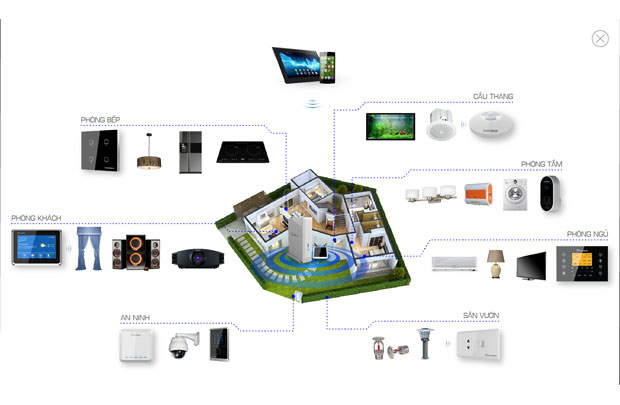
\includegraphics[scale=0.6]{images/overview.jpg}
    \caption{Overview of a Smart Home}
    \label{fig:overviewSmartHome}
    \end{center}
  \end{figure}

Besides, the house is usually implemented with sensors in order to collect environment data to maintain the best environment for the owner by controlling the devices such as conditioner, fan or curtains or to alert if a dangerous circumstance could happen.

\section{Current Research}
    With the rapidly growing of technology, especially connecting devices with the Internet becomes the trend today. Internet of Things is the combination of “things” including the new technology integrated thing or non-internet support thing but now is connected within the network, in order to connect and communicate to complete specified tasks.

    The connection between devices can be established via Wi-Fi, cellular network (3G, 4G and 5G in near future), Bluetooth, Zigbee or Infrared. The devices can be smartphones, circuit breakers, conditioner, headphones, light bulbs, and so on. The traditional devices (as they used to be) now can connect to the common network with a small integrated circuit with the function of establish any of connection mentioned above. However, letting a device running for 24 hours a day and 7 days a week is a real challenge because of their energy consumption, which is not solved effectively even in recent years.
    \subsection{Foreign Research}
    The giants in technology fields are already step into IoT field by providing services, software and hardware. For instance, Google introduced their Google Home with their voice recognition technology in order to automate the house activities. Beside Google, Amazon provides Amazon Echo and AWS with many integrated services which help their hardware products provided most satisfied experiences for the customers especially using Alex with trainable skill to control devices with voice recognition.

    In addition, there exists plenty of companies providing complete solution from hardware and extendable services to help with their products. For instance, Control4 is selling central device named EA series, focus on centralize control of devices and multimedia. Furthermore, their solution also included sensors integration in order to maintain the best environment for the users while using the house, such as dimming the light or pull curtains depends on day light insensitivity. 
    \subsection{Domestic Research}
    For domestic products, there are companies providing solutions based on foreign hardware in order to ensure the stability over time of the system. The company named Home Flow is an example who is providing the solutions and services based on Control4 and other foreign countries because Control4 products are opened source to ensure their partner can easily modify and extend their services. Moreover, there are companies that have strong potential of financial and research capability, namely Viettel or Bkav, they can research and introduce their own products. Thus, there is not yet remarkable products on the market by domestic companies.

\section{Thesis Objective}
In this thesis, the author only focus on implementing basic features for demonstration model with an advanced feature is Facial Recognition system embedded in a mini computer in order to run it without using a strong and costly personal computer, in which reduce the investment but still, achieve acceptable performance. The author will propose a centralize control model that can receive and distribute the command of controlling devices from distance by physical buttons in a flexible way and via Web Server with virtual buttons where user can control their devices from endless distance with the Internet Connection and a supported smart device. Last but not least, the thesis is also built in with a database in order to collect data for further development as data analysis is now becoming a serious trend along with the IoT applications.
\section{Thesis Structure}
This thesis consists of six chapters, in which are described as following.
\begin{itemize}
\item \textbf{Chapter 1}: Introduction of the project, which includes the idea of the author, project’s trend and some researches from foreign countries and also domestic ones.
\item \textbf{Chapter 2}: is the theory background of which the author read in order to collect appropriate knowledge to implement the project.
\item \textbf{Chapter 3}: is the hardware design, choosing components and sketch on Altium Designer with the overall hardware model.
\item \textbf{Chapter 4}: the software design for the system includes the algorithm of each implemented blocks.
\item \textbf{Chapter 5}: The results that the author achieved with real photos from the projects.
\item \textbf{Chapter 6}: Conclusion of the whole project with the limitations. In addition, the author also shows his future idea to improve the project.
\end{itemize}

